\documentclass[14pt]{extarticle}

\DeclareMathSizes{14}{14}{15}{12}

\renewcommand{\normalsize}{\fontsize{14}{16}\selectfont}


% Language setting
% Replace `english' with e.g. `spanish' to change the document language
\usepackage[english]{babel}
\usepackage{graphicx}
\graphicspath{ {./images/} }
% Set page size and margins
% Replace `letterpaper' with `a4paper' for UK/EU standard size

\usepackage[letterpaper,top=2cm,bottom=2cm,left=3cm,right=3cm,marginparwidth=1.75cm]{geometry}

% Useful packages
\usepackage{amsmath}
\usepackage{graphicx}
\usepackage[colorlinks=true, allcolors=blue]{hyperref}

\title{TP2 Automatique}

\begin{document}
\maketitle


\section{}

Soit $e(t)$ une impulsion de Dirac, $s(t)$ la réponse impulsionnelle du bloqueur d'ordre 0 et $u(t)$ le signal echelon unite. 


\[ s(t) = u(t) - u(t-T_e) \xrightarrow{\text{TL}} S(p) = \frac{1}{p} - \frac{e^{-pT_e}}{p} = \frac{1-e^{pT_e}}{p}\]
\[E(P) = 1\] 
\[B_0(P) = \frac{S(p)}{E(p)} = \frac{1-e^{pT_e}}{p}\] 


\section{}
\[A(z) = TZ[\frac{G_0(p)}{p}]\]
Dans le domaine temporel, on a :
\[TL^{-1}[\frac{G_0(p)}{p}] = TL^{-1}[\frac{1+p}{p^3}] = TL^{-1}[\frac{1}{p^2}] + TL^{-1}[\frac{1}{p^3}] = \frac{t^2}{2}u(t) + tu(t)\]

\[A(z) = TZ[\frac{t^2}{2}u(t) + tu(t)] = \frac{z(z+1)T_{e}^2}{2(z-1)^3} + \frac{zT_e}{(z-1)^2} = \frac{z(z+1)T_e^2+2z(z-1)T_e}{2(z-1)^3}\] 
\[G(z)= (1-z^{-1})A(z) = \frac{T_e(z(2+T_e)+T_e -2)}{2(z-1)^2}\]

\section{}

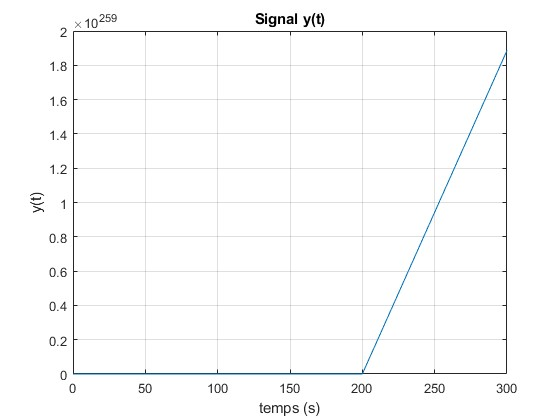
\includegraphics{untitled.jpg}

\section{}
\[H(z) = \frac{C(z)G(z)}{1+C(z)G(z)} = \frac{KT_e(z(2+T_e) + T_e - 2)}{2(z-1)^2 + KT_e(z(2+T_e)+T_e - 2)}\] 

Soit D(z) le polynome caracteristique au dénominateur de H(z) :
\[D(z) = 0 \Leftrightarrow 2(z-1)^2 + KT_e(z(2+T_e)+T_e - 2) = 0 \]

\[\Leftrightarrow 2z^2 + z(KT_e(2+T_e) - 4) + KT_e(T_e - 2) +2 = 0 \]

\end{document}
	
